% 第二章 理论基础
\chapter{理论基础}

\section{微磁学模型}

\subsection{连续介质近似}
微磁学（Micromagnetics）为纳米尺度磁性材料的磁化动力学分析提供了基本理论框架。该框架采用连续介质近似，将局域磁化矢量 $\mathbf{M}(\mathbf{r}, t)$ 的模约束为饱和磁化强度 $M_s$，并以单位矢量 $\mathbf{m}(\mathbf{r}, t) = \mathbf{M}/M_s$（满足 $|\mathbf{m}| = 1$）表征其空间取向。

体系总自由能 $E_{\text{total}}$ 包含若干独立的能量贡献项，具体如下。
\begin{equation}
  E_{\text{total}} = E_{\text{ex}} + E_{\text{DMI}} + E_{\text{anis}} + E_{\text{demag}} + E_{\text{Zeeman}}
  \label{eq:total-energy}
\end{equation}
上式右端各项依次对应交换能、Dzyaloshinskii-Moriya 相互作用（DMI）能、磁晶各向异性能、退磁能与塞曼能。

\subsection{交换相互作用}
海森堡交换相互作用促使相邻磁矩趋于平行排列。将该作用表述为连续介质形式，交换能可写作
\begin{equation}
  E_{\text{ex}} = \int A_{\text{ex}} \left[ (\nabla m_x)^2 + (\nabla m_y)^2 + (\nabla m_z)^2 \right] \, dV
  \label{eq:exchange}
\end{equation}
其中 $A_{\text{ex}}$ 为交换刚度常数，单位为 $\si{J/m}$。

阻挫交换体系的特殊之处在于，最近邻铁磁交换 $J_1 > 0$ 与次近邻反铁磁交换 $J_2 < 0$、第四近邻反铁磁交换 $J_4 < 0$ 共同作用。这种“受挫”交换机制能够为三维拓扑结构的稳定提供有效支撑\cite{sallermann2023stability}。

\subsection{Dzyaloshinskii-Moriya 相互作用}
DMI 属于反对称交换相互作用，其物理根源来自自旋-轨道耦合与空间反演对称性破缺的共同作用。在 DMI 影响下，相邻磁矩倾向于形成垂直取向，手性磁性拓扑结构的产生即以此为微观基础。

对于体积型（Bulk）DMI，能量密度为
\begin{equation}
  \varepsilon_{\text{DMI}}^{\text{bulk}} = D_{\text{bulk}} \, \mathbf{m} \cdot (\nabla \times \mathbf{m})
  \label{eq:dmi-bulk}
\end{equation}
在具备 B20 型晶体结构的 FeGe 或 MnSi 等手性磁体中，体积型 DMI 占据主导地位。

对于界面型（Interfacial）DMI，能量密度为
\begin{equation}
  \varepsilon_{\text{DMI}}^{\text{int}} = D_{\text{int}} \left( m_z \nabla \cdot \mathbf{m} - (\mathbf{m} \cdot \nabla) m_z \right)
  \label{eq:dmi-int}
\end{equation}
体积型与界面型 DMI 分别对应不同类型的拓扑磁构型，前者通常诱导产生 Bloch 型霍普夫子，后者则是形成 N\'{e}el 型霍普夫子的物理条件。

\subsection{磁晶各向异性}
单轴磁晶各向异性能量密度为
\begin{equation}
  \varepsilon_{\text{anis}} = K_{u1} (1 - m_z^2)
  \label{eq:anisotropy}
\end{equation}
其中 $K_{u1}$ 为一阶各向异性常数。当 $K_{u1} > 0$ 时，体系呈现沿 $z$ 轴的易轴各向异性，有利于维持均匀的背景磁化状态。需要指出的是，各向异性强度若超出临界值，霍普夫子 的尺寸将被持续压缩，最终导致结构湮灭。

\subsection{退磁场}
退磁场 $\mathbf{H}_{\text{demag}}$ 源于样品有限几何尺寸所引起的磁荷分布，可通过磁静力学方程求解。
\begin{equation}
  \nabla \cdot \mathbf{H}_{\text{demag}} = -\nabla \cdot \mathbf{M}
  \label{eq:demag}
\end{equation}
由于退磁场计算在微磁学求解过程中占用大量计算资源，Mumax3 采用快速傅里叶变换（FFT）算法以提升计算效率。数值仿真表明，在有限几何尺寸的样品中，退磁能是维持霍普夫子稳态结构的关键能量项。


\section{Landau-Lifshitz-Gilbert 方程}

磁化矢量随时间的演化行为遵循 Landau-Lifshitz-Gilbert（LLG）方程。
\begin{equation}
  \frac{\partial \mathbf{m}}{\partial t} = -\gamma_0 \, \mathbf{m} \times \mathbf{H}_{\text{eff}} + \alpha \, \mathbf{m} \times \frac{\partial \mathbf{m}}{\partial t}
  \label{eq:llg}
\end{equation}
其中 $\gamma_0 = \mu_0 |\gamma_e|$ 为旋磁比（$\gamma_e$ 为电子旋磁比），$\alpha$ 为 Gilbert 阻尼常数，$\mathbf{H}_{\text{eff}} = -\frac{1}{\mu_0 M_s}\frac{\delta E_{\text{total}}}{\delta \mathbf{m}}$ 为有效场。

LLG 方程刻画了磁化矢量的两类基本运动模式。其中进动项 $\mathbf{m} \times \mathbf{H}_{\text{eff}}$ 驱动磁化绕有效场做旋转运动，阻尼项则促使磁化逐步趋近有效场方向。微磁学模拟中常用的弛豫（Relax）操作，其物理本质等价于取 $\alpha \to \infty$ 的极限近似，由此使体系快速收敛至局域能量极小状态。

\subsection{自旋转移力矩}
当自旋极化电流流经磁性材料时，传导电子携带的自旋角动量向局域磁矩转移，产生自旋转移力矩（STT）。Zhang-Li 模型将 STT 分解为绝热分量与非绝热分量两个部分。
\begin{equation}
  \mathbf{T}_{\text{STT}} = -(\mathbf{u} \cdot \nabla)\mathbf{m} + \beta \, \mathbf{m} \times [(\mathbf{u} \cdot \nabla)\mathbf{m}]
  \label{eq:stt}
\end{equation}
其中 $\mathbf{u} = \frac{P j_e \mu_B}{e M_s}$ 为与电流密度成正比的速度矢量，$P$ 为自旋极化率，$\beta$ 为非绝热系数。


\subsection{自旋波与磁振子}
铁磁体达到平衡态后，全部磁矩呈平行排列。局域扰动一旦出现，受扰磁矩偏离平衡取向，经由交换耦合带动相邻磁矩协同进动，进而在空间中形成周期性的集体振荡，即自旋波（spin wave）。自旋波的能量量子化产物称为磁振子（magnon）。

对于零外加偏置场条件下的铁磁体，交换作用主导的自旋波色散关系具有如下形式。
\begin{equation}
  \omega_k = \gamma_0 \frac{2A_{\text{ex}}}{M_s} k^2
  \label{eq:sw-dispersion}
\end{equation}
其中 $k = |\mathbf{k}|$ 为波矢幅值，$2A_{\text{ex}}/M_s$ 为交换刚度参数。该色散关系呈抛物型特征，即波矢增大时自旋波频率随之升高，短波长磁振子对应更高的能量。

引入阻挫交换后，次近邻（$J_2 < 0$）与第四近邻（$J_4 < 0$）反铁磁交换项对色散关系产生实质性修正。在长波极限（$k \to 0$）区间内，铁磁交换 $J_1$ 仍居于主导地位，色散的抛物型特征基本不变；然而进入短波区域后，阻挫交换的影响使色散曲线显著偏离抛物线，并在特定波矢 $k^*$ 处形成凹陷极小值。
\begin{equation}
  k^* \approx \left(\frac{|J_2|}{J_1}\right)^{1/2} \frac{1}{a}
  \label{eq:sw-kstar}
\end{equation}
其中 $a$ 为格点间距。$k^*$ 处出现的磁振子软化现象与体系的螺旋不稳定性存在直接关联，霍普夫子 的特征长度尺度即由此确定。

微磁学仿真中，自旋波的激发通过在局域薄片区域施加随时间变化的磁场来实现。
\begin{equation}
  \mathbf{B}_{\text{sw}}(\mathbf{r}, t) = B_0 \sin(2\pi f_{\text{sw}} t) \cdot \hat{e} \cdot \chi(\mathbf{r})
  \label{eq:sw-excitation}
\end{equation}
其中 $B_0$ 为激发振幅，$f_{\text{sw}}$ 为驱动频率，$\hat{e}$ 为振荡极化方向，$\chi(\mathbf{r})$ 为源区域空间窗函数（取值 0 或 1）。仿真中在样品边界设置高阻尼吸收层，用以抑制反射波的干扰，从而等效地模拟半无限介质中自旋波的单向传播行为。

自旋波与三维磁性拓扑结构的相互作用机制是当前的重点研究方向\cite{liu2020three}。自旋波入射霍普夫子时的驱动效应主要来源于两个物理过程。第一是散射截面的空间不对称性引发的净辐射压力。第二是拓扑磁荷与自旋波角动量之间的直接耦合作用。后续数值分析证实，该耦合效率依赖于外加自旋波激发频率与振幅的协同调制，这也是第五章动力学仿真实验的核心变量。


\section{磁性霍普夫子的拓扑性质}

\subsection{Hopf 映射与 Hopf 指数}
霍普夫子 的拓扑性质植根于 Hopf 映射 $S^3 \to S^2$。三维空间经单点紧致化后拓扑等价于 $S^3$，磁化场 $\mathbf{m}(\mathbf{r})$ 将其映射至磁化方向空间 $S^2$。Hopf 指数由如下积分定义。
\begin{equation}
  Q_H = -\frac{1}{4\pi^2} \int \mathbf{F} \cdot \mathbf{A} \, d^3r
  \label{eq:hopf-index}
\end{equation}
其中 $\mathbf{F}$ 为涌现电磁场张量，$\mathbf{A}$ 为对应的矢量势。$Q_H$ 是整数拓扑不变量，$Q_H = 1$ 对应最简单的 霍普夫子。

\begin{figure}[H]
  \centering
  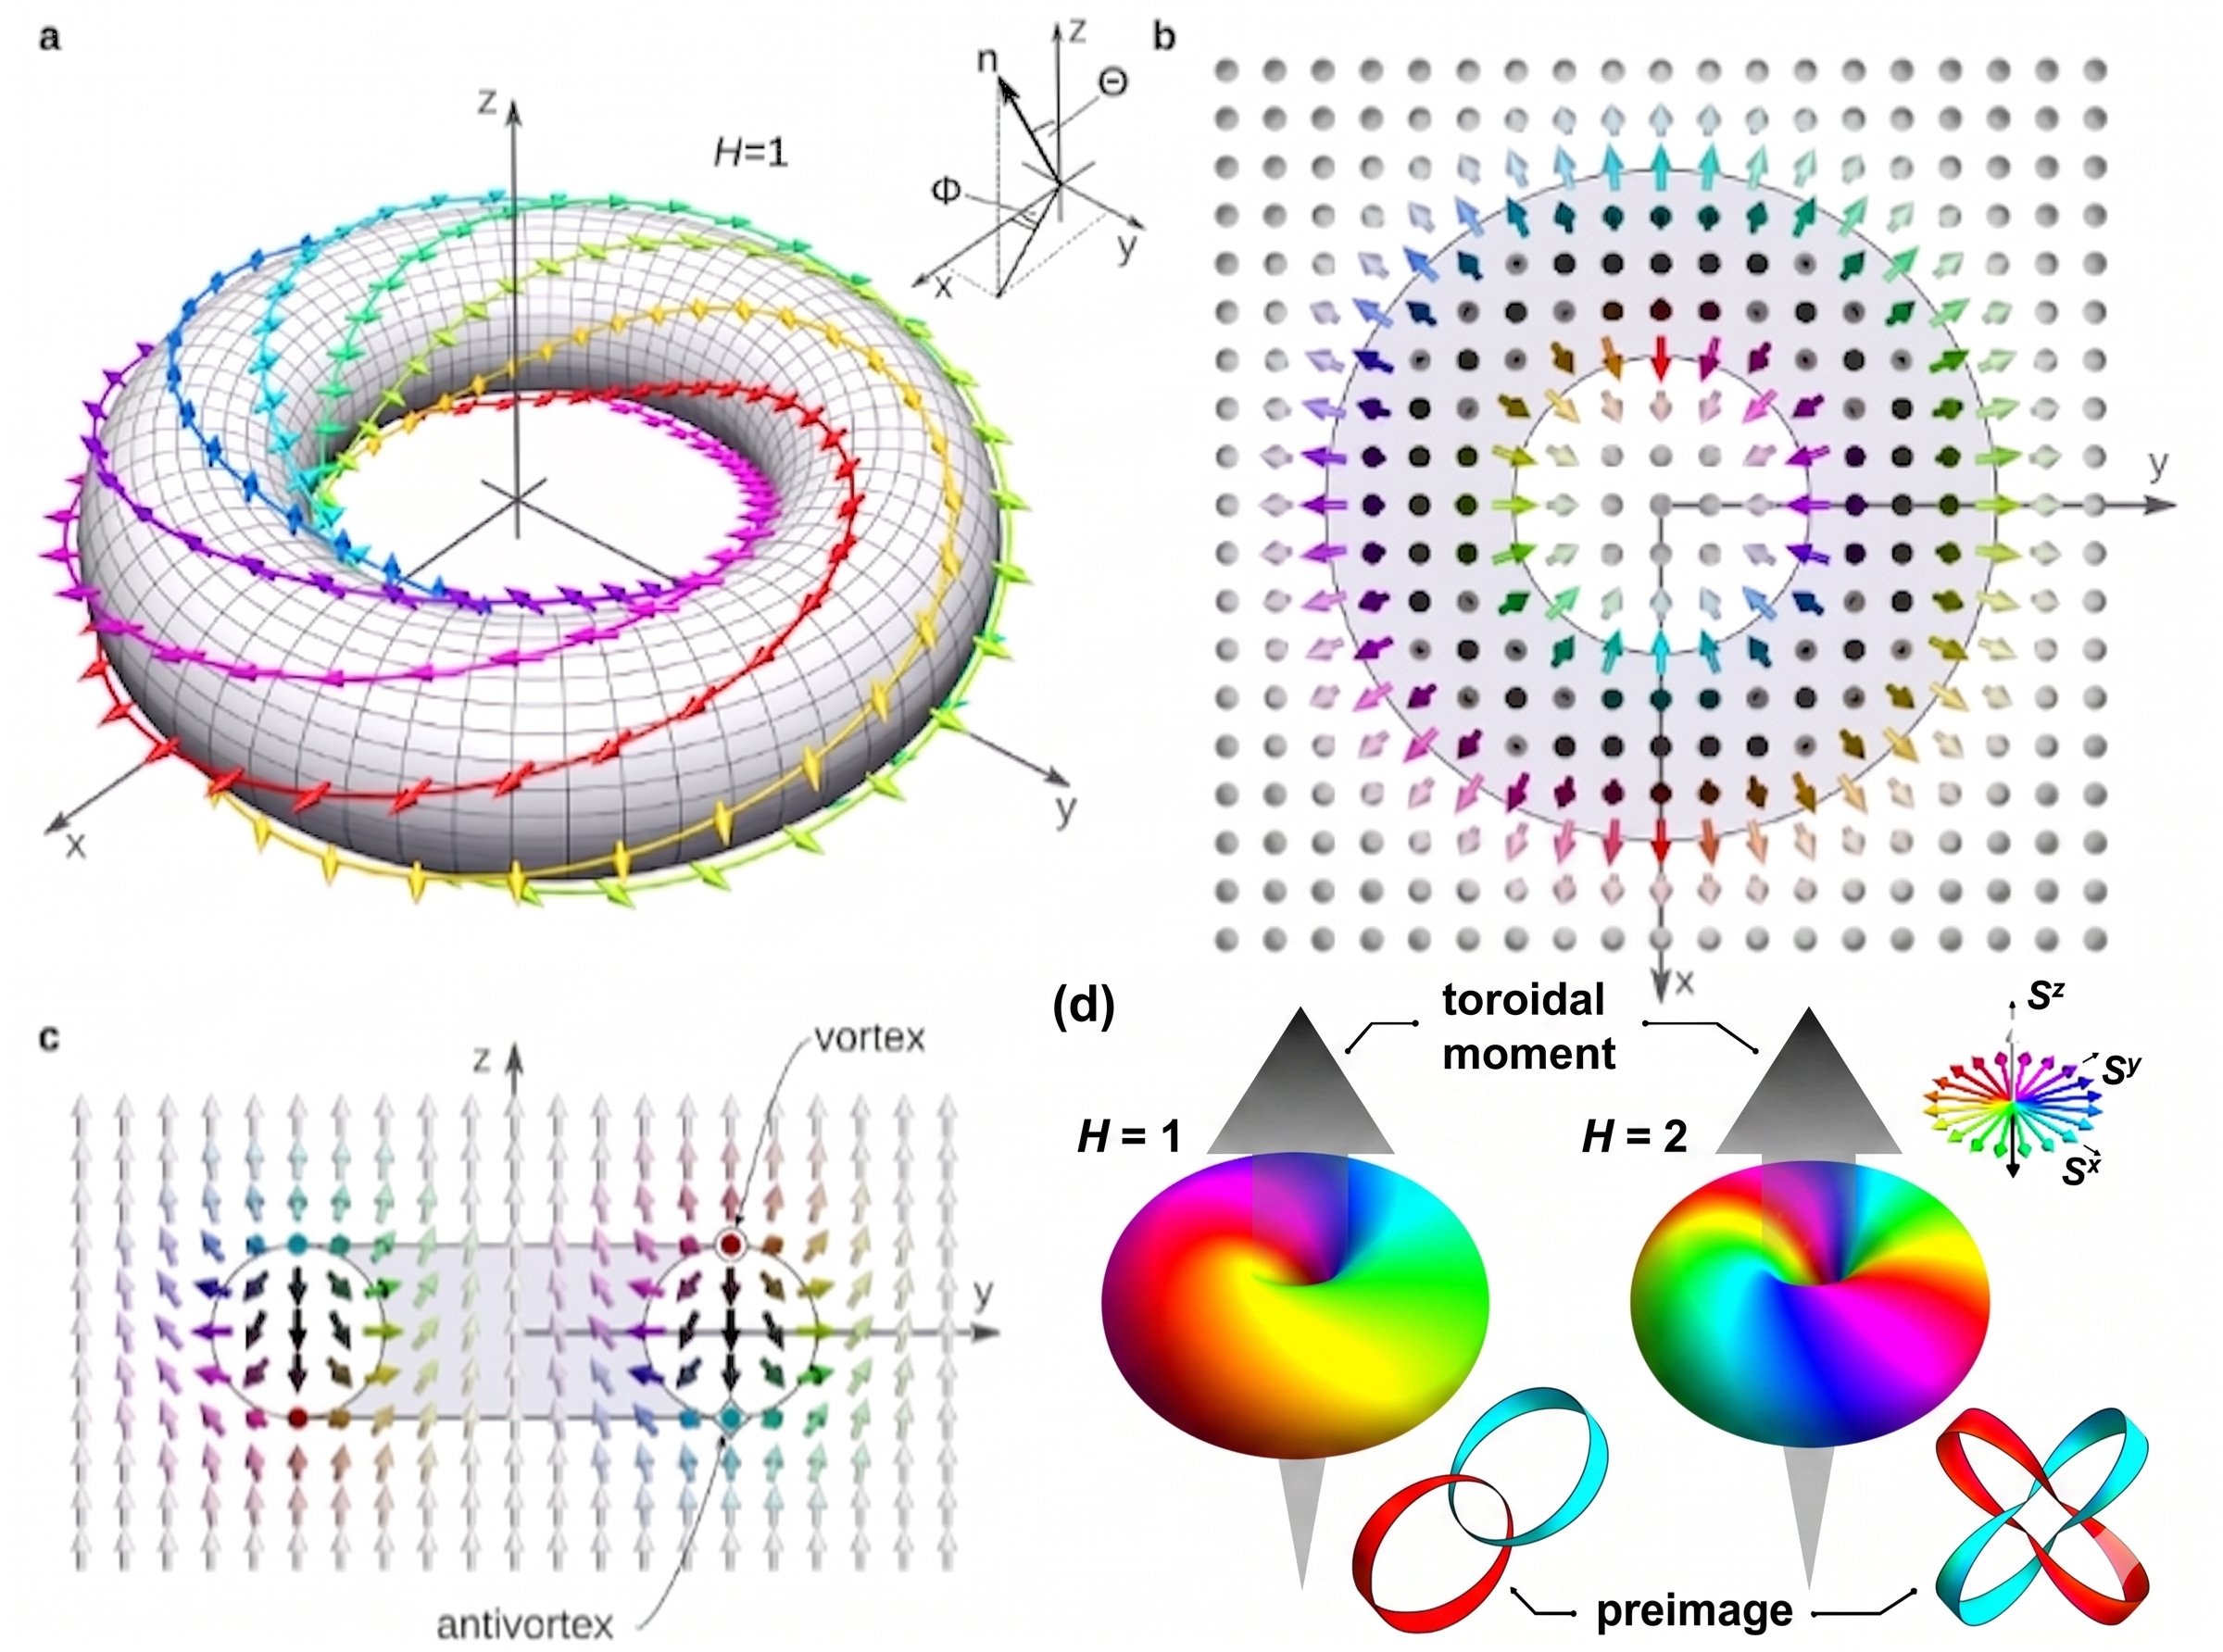
\includegraphics[width=0.85\textwidth]{figures/fig2-1_hopfion_preimage_view.png}
  \caption[霍普夫子的三维构型、面内切面与环面动量]{霍普夫子 的三维磁化构型与几何刻画。(a) $H = 1$ 霍普夫子 的环面几何与表面磁化分布，前像 沿管轴方向螺旋缠绕；(b) 过环面中心的 $xy$ 切面，面内磁化呈双涡旋结构；(c) 沿 $yz$ 切面的磁化分布，可见涡旋–反涡旋对\cite{rybakov2022magnetic}。(d) $H = 1$ 与 $H = 2$ 环面动量及其 前像 缠绕链接示意\cite{kasai2025sot}。}
  \label{fig:hopfion-core-schematic}
\end{figure}

\subsection{霍普夫子的物理结构}
以最简单的 $H = 1$ 霍普夫子 为例，其构型可借助甜甜圈几何加以直观描述。甜甜圈本体对应磁矩朝下（$m_z = -1$）的环形核心，甜甜圈之外的样品区域为磁矩朝上（$m_z = +1$）的均匀背景；两者之间存在一层过渡层，层内磁矩方向沿甜甜圈表面逐点平滑旋转，将朝下与朝上两种取向连续衔接起来，整体形成三维纽结几何。为刻画该环面尺寸，定义大半径 $R$ 为环面中心轴到管截面圆心的距离，管半径 $r$ 为管截面圆的半径，二者满足 $R > r$。\cref{fig:hopfion-core-schematic}(b) 给出过环面中心的 $xy$ 切面，其中左右两个手性相反的涡旋对应管截面被切开后的两段，涡旋中心间距即 $2R$，单个涡旋的径向尺寸则对应 $2r$；\cref{fig:hopfion-core-schematic}(c) 给出 $yz$ 切面，涡旋–反涡旋对清晰可辨，反映了反向磁化管在轴向被截断后的磁化投影形貌。$R$ 刻画核心环的主周长尺度，$r$ 决定过渡层的径向厚度，二者是 霍普夫子 几何状态的最紧凑描述，亦构成后续稳定性与动力学分析的主要观测量。

前像是把握 霍普夫子 拓扑本质的核心概念。对磁化方向空间 $S^2$ 上任意一点，其 前像 定义为三维实空间中所有磁化矢量指向该方向的位置所构成的集合，通常形成一条闭合曲线。\cref{fig:hopfion-core-schematic}(d) 下方用两条着色闭环示意了分别对应不同磁化方向的 前像，它们在空间中相互缠绕而非彼此分离；缠绕的链接数即为 Hopf 指数 $H$（亦记作 $Q_H$）。换言之，$H$ 的拓扑意义不在磁化场本身的强度或方向，而在于不同方向 前像 闭环之间的链接数，也就是任意两条闭环相互穿过的次数。

$H$ 值的直观含义可由\cref{fig:hopfion-core-schematic}(d) 上方的球面磁化分布读出。$H = 1$ 对应最基本的单环面构型，磁化方向沿环面一圈即完成一次 $S^2$ 覆盖，下方两条 前像 闭环仅相互穿越一次；$H = 2$ 则表现为球面上磁化方向扭转次数加倍的更密构型，下方两条 前像 相互缠绕两次、链接数随之翻倍。由此可以看出，$H$ 值越高，磁化场在空间中的扭结程度越强，对应的能量代价与稳定门槛亦随之抬升，这也解释了高阶 霍普夫子 在数值实验中更易坍塌的现象。

\section{Mumax3 仿真平台}

Mumax3 是由根特大学 DyNaMat 课题组开发的开源微磁学模拟软件\cite{vansteenkiste2014design}，以有限差分方法在正交均匀网格上离散 LLG 方程，并通过 GPU 并行完成三维磁化动力学求解。单元立方体中心存储单位磁化矢量 $\mathbf{m}_i$，交换、各向异性、塞曼与 DMI 等有效场贡献以局域差分形式求值，退磁场通过快速傅里叶变换加速卷积；时间积分默认采用多曼德–普林斯自适应龙格–库塔法（RK45），弛豫场景则使用内置能量最小化器加速收敛。

仿真由 Go 风格脚本（.mx3）驱动，磁化构型以 .ovf 格式按节点输出，宏观物理量写入 table.txt。本文在此基础上扩展了若干自定义观测量，包括 Hopf 指数 $Q_H$、霍普夫子 质心坐标以及大半径 $R$、管半径 $r$ 的在线提取，全部实时写入 table.txt，以降低 .ovf 文件的事后分析开销。

本文全部微磁学模拟均在 Mumax3 v3.11.1 下完成，计算任务分布在两台机器，其中一台为搭载 NVIDIA RTX 5070 Ti Laptop GPU 的本地笔记本，另一台为杭州电子科技大学第三教学楼 519 实验室内配置 NVIDIA GeForce RTX 2080 Ti GPU 的工作站；两者均运行 CUDA 12.x 环境，同一脚本在双平台上输出在机器精度内一致。
